\documentclass[ucs,9pt]{beamer}

% Copyright 2004 by Till Tantau <tantau@users.sourceforge.net>.
%
% In principle, this file can be redistributed and/or modified under
% the terms of the GNU Public License, version 2.
%
% However, this file is supposed to be a template to be modified
% for your own needs. For this reason, if you use this file as a
% template and not specifically distribute it as part of a another
% package/program, I grant the extra permission to freely copy and
% modify this file as you see fit and even to delete this copyright
% notice.
%
% Modified by Tobias G. Pfeiffer <tobias.pfeiffer@math.fu-berlin.de>
% to show usage of some features specific to the FU Berlin template.

% remove this line and the "ucs" option to the documentclass when your editor is not utf8-capable
\usepackage[utf8x]{inputenc}    % to make utf-8 input possible
\usepackage[english]{babel}     % hyphenation etc., alternatively use 'german' as parameter

% Template for talks using the Corporate Design of the Freie Universitaet
%   Berlin, created following the guidelines on www.fu-berlin.de/cd by
%   Tobias G. Pfeiffer, <tobias.pfeiffer@math.fu-berlin.de>
% This file can be redistributed and/or modified in any way you like.
%   If you feel you have done significant improvements to this template,
%   please consider providing your modified version to
%   https://www.mi.fu-berlin.de/w/Mi/BeamerTemplateCorporateDesign

\usepackage{amsmath,dsfont,listings}

%%% FU logo
% small version for upper right corner of normal pages
\pgfdeclareimage[height=0.9cm]{university-logo}{FULogo_RGB}
\logo{\pgfuseimage{university-logo}}
% large version for upper right corner of title page
\pgfdeclareimage[height=1.085cm]{big-university-logo}{FULogo_RGB}
\newcommand{\titleimage}[1]{\pgfdeclareimage[height=2.92cm]{title-image}{#1}}
\titlegraphic{\pgfuseimage{title-image}}
%%% end FU logo

% NOTE: 1cm = 0.393 in = 28.346 pt;    1 pt = 1/72 in = 0.0352 cm
\setbeamersize{text margin right=3.5mm, text margin left=7.5mm}  % text margin

% colors to be used
\definecolor{text-grey}{rgb}{0.45, 0.45, 0.45} % grey text on white background
\definecolor{bg-grey}{rgb}{0.66, 0.65, 0.60} % grey background (for white text)
\definecolor{fu-blue}{RGB}{0, 51, 102} % blue text
\definecolor{fu-green}{RGB}{153, 204, 0} % green text
\definecolor{fu-red}{RGB}{204, 0, 0} % red text (used by \alert)

% switch off the sidebars
% TODO: loading \useoutertheme{sidebar} (which is maybe wanted) also inserts
%   a sidebar on title page (unwanted), also indents the page title (unwanted?),
%   and duplicates the navigation symbols (unwanted)
\setbeamersize{sidebar width left=0cm, sidebar width right=0mm}
\setbeamertemplate{sidebar right}{}
\setbeamertemplate{sidebar left}{}
%    XOR
% \useoutertheme{sidebar}

% frame title
% is truncated before logo and splits on two lines
% if neccessary (or manually using \\)
\setbeamertemplate{frametitle}{%
    \vskip-30pt \color{text-grey}\large%
    \begin{minipage}[b][23pt]{80.5mm}%
    \flushleft\insertframetitle%
    \end{minipage}%
}

%%% title page
% TODO: get rid of the navigation symbols on the title page.
%   actually, \frame[plain] *should* remove them...
\setbeamertemplate{title page}{
% upper right: FU logo
\vskip2pt\hfill\pgfuseimage{big-university-logo} \\
\vskip6pt\hskip3pt
% title image of the presentation
\begin{minipage}{11.6cm}
\hspace{-1mm}\inserttitlegraphic
\end{minipage}

% set the title and the author
\vskip14pt
\parbox[top][1.35cm][c]{11cm}{\color{text-grey}\inserttitle \\ \small \insertsubtitle}
\vskip11pt
\parbox[top][1.35cm][c]{11cm}{\small \insertauthor \\ \insertinstitute \\[3mm] \insertdate}
}
%%% end title page

%%% colors
\usecolortheme{lily}
\setbeamercolor*{normal text}{fg=black,bg=white}
\setbeamercolor*{alerted text}{fg=fu-red}
\setbeamercolor*{example text}{fg=fu-green}
\setbeamercolor*{structure}{fg=fu-blue}

\setbeamercolor*{block title}{fg=white,bg=black!50}
\setbeamercolor*{block title alerted}{fg=white,bg=black!50}
\setbeamercolor*{block title example}{fg=white,bg=black!50}

\setbeamercolor*{block body}{bg=black!10}
\setbeamercolor*{block body alerted}{bg=black!10}
\setbeamercolor*{block body example}{bg=black!10}

\setbeamercolor{bibliography entry author}{fg=fu-blue}
% TODO: this doesn't work at all:
\setbeamercolor{bibliography entry journal}{fg=text-grey}

\setbeamercolor{item}{fg=fu-blue}
\setbeamercolor{navigation symbols}{fg=text-grey,bg=bg-grey}
%%% end colors

%%% headline
\setbeamertemplate{headline}{
\vskip4pt\hfill\insertlogo\hspace{3.5mm} % logo on the right

\vskip6pt\color{fu-blue}\rule{\textwidth}{0.4pt} % horizontal line
}
%%% end headline

%%% footline
\newcommand{\footlinetext}{\insertshortinstitute, \insertshorttitle} %, \insertshortdate}
\setbeamertemplate{footline}{
\vskip5pt\color{fu-blue}\rule{\textwidth}{0.4pt}\\ % horizontal line
\vskip2pt
\makebox[123mm]{\hspace{7.5mm}
\color{fu-blue}\footlinetext
\hfill \raisebox{-1pt}{\usebeamertemplate***{navigation symbols}}
\hfill \insertframenumber}
\vskip4pt
}
%%% end footline

%%% settings for listings package
\lstset{extendedchars=true, showstringspaces=false, basicstyle=\footnotesize\sffamily, tabsize=2, breaklines=true, breakindent=10pt, frame=l, columns=fullflexible}
\lstset{language=Java} % this sets the syntax highlighting
\lstset{mathescape=true} % this switches on $...$ substitution in code
% enables UTF-8 in source code:
\lstset{literate={ä}{{\"a}}1 {ö}{{\"o}}1 {ü}{{\"u}}1 {Ä}{{\"A}}1 {Ö}{{\"O}}1 {Ü}{{\"U}}1 {ß}{\ss}1}
%%% end listings  % THIS is the line that includes the FU template!

\usepackage{arev,t1enc} % looks nicer than the standard sans-serif font
% if you experience problems, comment out the line above and change
% the documentclass option "9pt" to "10pt"

% image to be shown on the title page (without file extension, should be pdf or png)
\titleimage{fu_500}

\title[Privacy and Security Threats of IoT Wearables] % (optional, use only with long paper titles)
{Smartwatches and Fitness trackers: Cyberphysical Privacy and Security Threats}

\subtitle
{IoT and Security}

\author[Author, Another] % (optional, use only with lots of authors)
{Henrik Strangalies} % F.~Author \and S.~Another
% - Give the names in the same order as the appear in the paper.

\institute[Computer Science] % (optional, but mostly needed)
{Freie Universität Berlin}
% - Keep it simple, no one is interested in your street address.

%\date[CFP 2003] % (optional, should be abbreviation of conference name)
%{Conference on Fabulous Presentations, 2003}
% - Either use conference name or its abbreviation.
% - Not really informative to the audience, more for people (including
%   yourself) who are reading the slides online

\subject{Technical Computer Science}
% This is only inserted into the PDF information catalog. Can be left
% out.

% you can redefine the text shown in the footline. use a combination of
% \insertshortauthor, \insertshortinstitute, \insertshorttitle, \insertshortdate, ...
\renewcommand{\footlinetext}{\insertshortinstitute, \insertshorttitle, \insertshortdate}

% Delete this, if you do not want the table of contents to pop up at
% the beginning of each subsection:
\AtBeginSubsection[]
{
  \begin{frame}<beamer>{Outline}
    \tableofcontents[currentsection,currentsubsection]
  \end{frame}
}

\begin{document}

\begin{frame}[plain]
  \titlepage
\end{frame}

\begin{frame}{Outline}
  \tableofcontents
  % You might wish to add the option [pausesections]
\end{frame}

\section{Motivation}



\begin{frame}{Motivation behind IoT wearables: Smartwatches and Fitness Trackers}
  % - A title should summarize the slide in an understandable fashion. 
  %   for anyone how does not follow everything on the slide itself.
  \begin{itemize}
  \item Wearable devices have become increasingly popular
   due to their convenience and functionality.
  \item Enabling users to perform various tasks such as \textbf{making payments}, \textbf{monitoring health}, and \textbf{receiving messages}.
  
  \begin{figure}
  	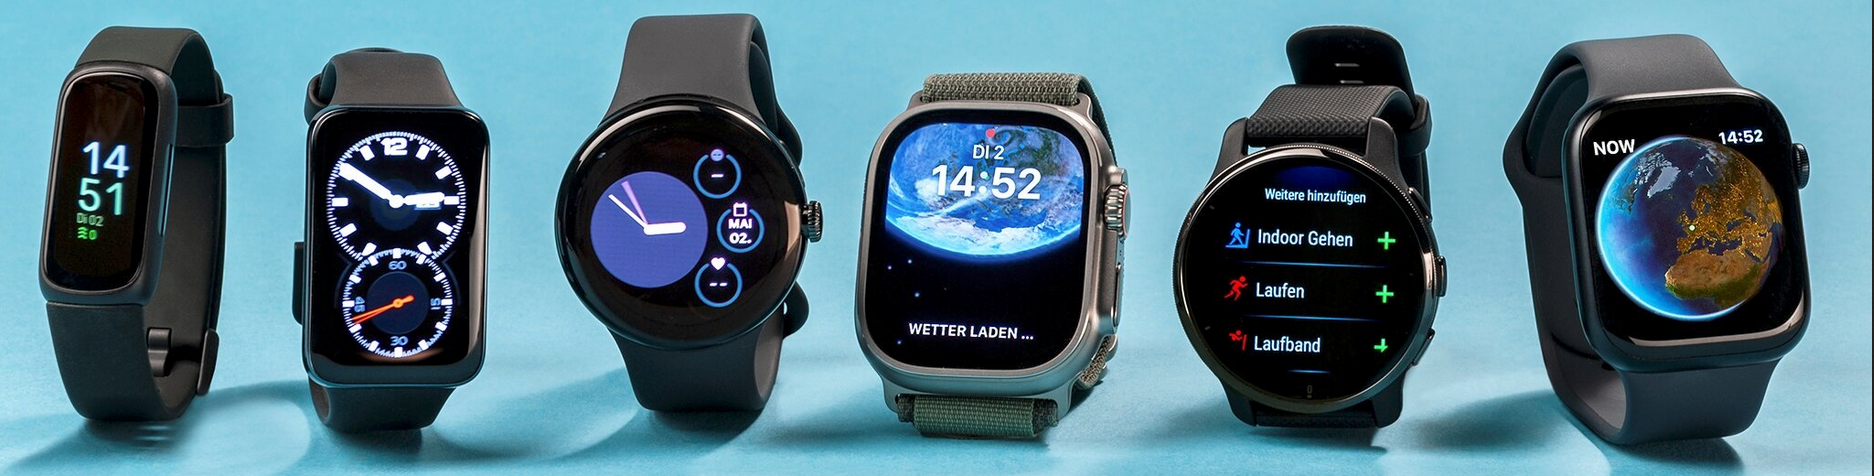
\includegraphics[width=\linewidth]{imgs/smartwatches}
  	\caption{Figure is taken from \cite{smartwatches}.}
  \end{figure}
  
  \pause 
  
  \item  Along with these benefits, wearables bring forth security and privacy concerns:
  \begin{itemize}
	\item \textbf{Data Collection.}
	\item \textbf{Data Transfer} between wearable device and phone.
	\item Applications of \textbf{third-party companies}.
	\item Location-based threats.
  \end{itemize}
  \end{itemize}
\end{frame}


\section{Panorama of Security \& Privacy Considerations with IoT wearables}

\begin{frame}[fragile]{Panorama of Security \& Privacy Considerations with IoT wearables}

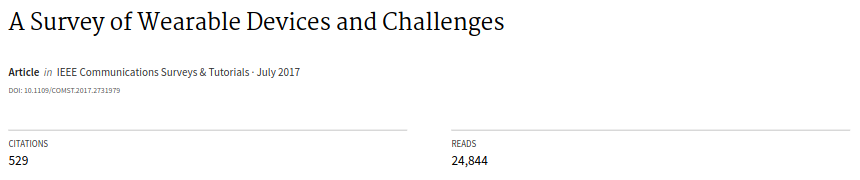
\includegraphics[width=1\linewidth]{imgs/ASurveyofWearableDevicesandChallenges}

\end{frame}


\subsection{Threats to Confidentiality}

\begin{frame}{Confidentiality}
	\begin{alertblock}{Definition}
	Threats to Confidentiality encompasses those where attackers get unauthorised  access to information using techniques such as eavesdropping  the wireless channel.	
	\end{alertblock}
	
	% 	Most existing wearable devices use Bluetooth Low Energy (BLE) as the major means of communication.
	
	
\end{frame}

\begin{frame}{Eavesdropping}
	\begin{itemize}
		\item Eavesdropping is the unauthorized real-time interception of a private communication which can expose user’s personal information to an attacker.
%Particularly, wearable devices using BLE communication protocol can suffer from eavesdropping.	
		\item The authors of the Open Effect Report from 2016 \cite{b7} investigated BLE privacy provision in number of fitness tracking devices such as Fitbit Charge HR, Jawbone UP 2, Garmin Vivosmart, 	Apple Watch, and Xiaomi Mi Band and came to the conclusion all tested devices, except Apple Watch, use the static device addresses that allowed attackers to \textbf{track user information such as location, time of fitness activities, and reversing user profile} by eavesdropping on these devices’ communications.
	\end{itemize}
\end{frame}

\begin{frame}{Traffic analysis}
	\begin{itemize}
		\item Traffic analysis attacks in the context of wearables involve monitoring communication patterns between devices.
		\item Privacy vulnerabilities have been identified in Bluetooth Low Energy (BLE) communication between fitness trackers and smartphones. 
		\item Adversaries can track users by analyzing BLE advertisements and static device addresses. 
		\item User activities can be inferred from the size and number of data packets in BLE traffic, even if the packets are encrypted. 
		\item Unique walking patterns can also be used to identify individuals within a small group, even with random 	addresses [1].
		\item It has been shown that the majority of fitness 		trackers use unchanged BLE addresses during advertising, 		making it feasible to track them. 
		\item The BLE traffic of the 		fitness trackers is found to be correlated with the intensity 		of the user’s activity, enabling an eavesdropper to determine 		the \textbf{user’s current activity} (walking, sitting, idle, or running) 		through analysis of the BLE traffic. 
	\end{itemize}
\end{frame}

\begin{frame}{Infomration Gathering Attacks.}
	\begin{itemize}
		\item Passive monitoring of wearable device transmissions enables adversaries to collect data exchanged between wearables and their hubs. 
		\item This information can be used for information gathering attacks, including breaking key exchanges in Bluetooth Low Energy (BLE) pairing and gathering information about user's other devices. 
		\item Researchers have demonstrated attacks that break BLE legacy pairing, infer keystrokes on smartphone touchpads using smartwatch motion sensors, decode keystrokes on keyboards using smartwatch sensors, and infer a user's personal PIN sequence using wearable devices.
		\item Adversaries can gain access to smartwatches by installing malicious applications to record sensor activities. 
		\item These attacks leverage sensor data captured by wearables and can be executed by sniffing BLE communications or installing malicious apps on wearables \cite{b1}.
	\end{itemize}
\end{frame}


\subsection{Threats to Integrity}


\begin{frame}{Threats to Integrity}
	\begin{alertblock}{Definiton}
		Threats to Integrity includes the cases  where attackers alter data or information without authorisation.  Threats to Availability are the situations where attackers act  to deny services to the entities who are authorised to use them.
	\end{alertblock}
	
	%Integrity is a crucial security requirement for wearable systems, particularly due to the sensitivity and privacy of the collected data. 	
	%Ensuring that data remains unaltered during transmission and reaches only authorized parties is paramount.	 
	%Various studies in the literature have evaluated the integrity of 		wearable device systems, identifying vulnerabilities in three attack categories: Modification Attacks, Replay Attacks, and Masquerade Attacks [1]. Additionally, this section comprises an overview of possible data breaches.
\end{frame}



\begin{frame}{Modification Attacks}
	\begin{itemize}
		\item In wireless data transmission between wearable devices, there is a risk of data modification or alteration. 
		\item Adversaries can intercept and modify data exchanged between wearable devices, including changing packet content and timestamps. Vulnerabilities have been found in Bluetooth LE pairing, fitness data storage, and transmission in popular trackers such as FitBit and Garmin.
		\item Attackers can exploit these vulnerabilities to capture, modify, and inject data. 
		\item Timestamp integrity in healthcare devices has also been compromised, allowing attackers to tamper with medical data.
		\item The lack of HTTPS transmission in certain applications exposes sensitive fitness data to unauthorized parties, enabling data falsification.
	\end{itemize}
\end{frame}

\begin{frame}{Replay Attacks}
	\begin{itemize}
		\item In replay attacks, adversaries capture valid data packets uploaded by a wearable device and replay them for malicious purposes such as impersonation or data corruption. 
		\item A notable example was mentioned where  a replay attack was demonstrated in a commercially available insulin delivery system.
		\item By eavesdropping on the communication between devices, attackers can gather information transmitted in plaintext, including device type, PIN, therapy or glucose level, and patient's medical condition. 
		\item Through brute-force methods, they can determine the Cyclic Redundant Check parameters used in the system and perform replay attacks by altering the counter field of the packet, reporting outdated glucose levels as an example.
	\end{itemize}
\end{frame}

\begin{frame}{Masquerade Attacks}
	\begin{itemize}
		\item Masquerade attacks involve impersonating an authenticated device to steal data or inject fake information. 
		\item Examples include collecting bonding information from medical devices through malicious apps and controlling insulin pumps by knowing the device's PIN.
		\item  These attacks exploit the lack of authentication and encryption in wearable systems. 
		\item While threats to integrity are less common than those to confidentiality, addressing data confidentiality vulnerabilities will also protect data integrity.
	\end{itemize}
\end{frame}




\begin{frame}{Data Breaches}
	\begin{itemize}
		%Wearable manufacturers commonly offer companion mobile applications that can be installed on smartphones to enhance the functionality and user experience of the wearable devices. These applications serve as a communication interface between the wearable device and the smartphone, allowing users to access and interact with a wide range of features and data. 
		% 	Indeed, data collection is paramount for providing users with plenty features to track theirs health and lead to a healthy lifestyle.  On the other hand, the massive data collection is prune for data breaches.
		
		\item Smartwatches and fitness tracker bracelets can provide measurements such as distance walked or run using motion sensors and GPS.
		\item  They can also monitor physiological/biological parameters like heart rate, ECG, stress levels, sleep quality, and more.
		% The mobile applications provide a comprehensive user interface to visualize, analyze, and manage this data, offering users a holistic view of their health and activity information.  
		
		\item Heart-related metrics and polysomnographic parameter can be measured due to optical sensors are commonly integrated into smartphones and smartwatches to detect variations in blood volume within the arteries beneath the skin.
		
		\item It has been shown that the identification of various activities such as stationary behavior, walking, running, bicycling, stair climbing, descent, and driving was achieved solely through the utilization of accelerometer data. 		
		\item Information pertaining to sleep, including sleep posture and habits, has been successfully extracted using motion sensors. 		
		\item A study employed accelerometer, gyroscope, and orientation data from a smartwatch to detect sleep posture and hand position during sleep.
	\end{itemize}
\end{frame}


\subsection{Threats to Availability}

\begin{frame}{Threats to Availability}
	
	\begin{alertblock}{Definiton}
		Threats to Availability are the situations where attackers act  to deny services to the entities who are authorized to use them.
	\end{alertblock}
\end{frame}

\begin{frame}{Threats to Availability}
	\begin{itemize}
		\item Denial of Service (DoS) attacks are a common type of attack against availability in wearable devices. 
		\item They aim to disrupt communication between wearables and their base or overwhelm the device's storage capacity with useless information. 
		%Examples of such attacks have been documented in the research literature.
		\item For instance, the FitBit Charge tracker can be targeted with DoS attacks to prevent legitimate device syncing or pairing with mobile phones.
		\item Attack tools like Fitbite and GarMax have been used to inject fake data, exceeding the storage capacity of trackers, thereby preventing them from recording valid user data.
		\item These attacks can drain the battery by continuously querying the nearby trackers. 
		%It is important for manufacturers to address these implementation shortcomings in future wearable products, especially in critical healthcare devices like insulin pumps that require uninterrupted functionality. Continuous vigilance and vulnerability assessments are crucial to ensure the availability of wearable systems \cite{b1}
	\end{itemize}
\end{frame}



\section{Threats to security and privacy from accelerometer data}


\begin{frame}[fragile]{Threats to security and privacy from accelerometer data}
	
	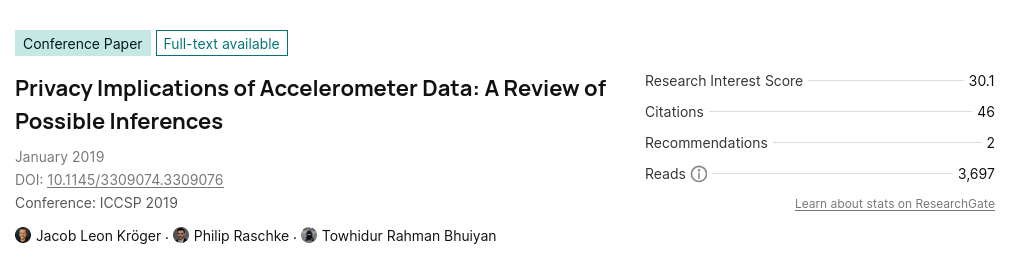
\includegraphics[width=1\linewidth]{imgs/Privacy Implications of Accelerometer Data A Review of Possible Inferences}
	
	% Particularly, privacy and security risks arise from the collection and utilization of accelerometer data on smartwatches and 	fitness trackers. The accelerometer, which measures motion 	and movement, can inadvertently disclose sensitive information about an individual’s activities and behavior. 
	% This data, if not properly protected, can be accessed by unauthorized parties and potentially lead to privacy or security breaches. Safeguarding the privacy of accelerometer data is crucial to ensure the confidentiality and security of users' personal information. 	The paper by Kröger et al. \cite{b5} is predestined for exemplifying that topic, since it highlights the potential privacy implications of accelerometers and security aspects such as inferring passwords, which are commonly found in mobile devices. While accelerometers are generally considered non-intrusive and do not require special permissions, research has shown that they can be used as a side channel to infer sensitive information about device holders. Accelerometer data alone can reveal details such as location, activities, health condition, body features, gender, age, personality traits, and emotional state. It can even be used for biometric identification and reconstructing text sequences, including passwords.
\end{frame}


\begin{frame}{Activity And Behavior Tracking}
% Accelerometers provide valuable data for a wide range of applications and can derive various physical activity variables and behavior-related information.
\begin{itemize}
	\item Accelerometers are used in step counters to estimate \textbf{energy expenditure} and \textbf{distance walked}, and in medical studies to assess \textbf{sedentary time and physical activity}.
	\item They enable real-time \textbf{body posture} and \textbf{activity
	classification}, including basic activities like running, walking,
	and sitting, as well as more complex activities like writing,
	typing, and painting. 
	\item They can also monitor \textbf{sleep patterns
	and behaviors}. 
	\item They can detect \textbf{hand 	gestures, eating and drinking moments, smoking, and even
	distinguish levels of intoxication}. 
	\item They have been used to detect \textbf{carried loads and estimate carried weight}, \textbf{measure driving behavior}, \textbf{analyze speech activity} and \textbf{social interactions}, and
	\textbf{reconstruct speech from recorded vibrations}. 
	%\item It has been observed that researchers were able to detect aggressive or 	unsafe driving styles and drunk driving patterns. 
 	% The potential applications of accelerometers are vast and extend to various	domains such as healthcare, fitness tracking, and behavior 	analysis [5].
\end{itemize}
\end{frame}


\begin{frame}{Location Tracking}
\begin{itemize}
	\item Studies have demonstrated that accelerometers in mobile
	devices can be utilized for \textbf{user localization and reconstruction
	of travel trajectories}, even in the absence of GPS or other localization systems.
	\item Researchers have achieved \textbf{geographically tracking individuals driving a car} solely based on accelerometer readings from their smartphones.
%  By analyzing three-axis acceleration measurements and mapping them to existing 	routes on a map, they obtained trajectory information with accuracy comparable to handheld GPS devices. 
	\item Another study focused on using smartphone accelerometers to determine the \textbf{location of the user within a metropolitan train system}. 
	%By comparing acceleration patterns with labeled training data, specific station intervals were recognized, and the accuracy	of the approach reached up to 89% for rides longer than 3 stations and 92% for rides longer than 5 stations. These 	findings highlight the potential privacy risks associated with 	accelerometer data and the ability to infer sensitive information about individuals’ whereabouts and travel patterns [5].
\end{itemize}
\end{frame}


\begin{frame}{User Identification}
\begin{itemize}
	\item Ability to differentiate between and uniquely identify users
	\textbf{based on their body movement patterns}. 
	\item Biometric features such as \textbf{gait, hand gestures, and head movements}  have been used for user identification with high
	accuracy. % For example, one study achieved 100% accuracy in recognizing individuals from a test group using accelerometer readings from smartphones. 
	\item Capability distinguish between different speakers accurately by sound vibrations, including human speech, with enough quality to .
	\item The trajectory of a mobile device can reveal a \textbf{user’s work and home addresses}. 
	\item When combined with other auxiliary datasets, such as white pages
	or employment directories, it can potentially expose a user’s
	real identity.
	%\item Device fingerprinting techniques can further differentiate users based on unique characteristics of their personal devices. 
	\item Calibration errors in accelerometers %, caused by manufacturing imperfections,
	have been found sufficient to create a device ”fingerprint” that can track users across website visits, even when other tracking technologies like cookies are
	blocked.
\end{itemize}
\end{frame}


\begin{frame}{Keystroke Logging}
  \begin{itemize}
  	\item The input that users type into their devices, whether through touchscreens or keyboards, often contains highly sensitive information such as text messages, personal notes, login credentials, and transaction details. 
  	% Researchers have shown that motion sensor data can be used to reconstruct user inputs from handheld and wrist-worn devices.
  	%By analyzing the hand movements associated with swipes, taps, and keystrokes, researchers have successfully inferred inputs from motion sensor data. 
  	\item Researchers have demonstrated to infer tap- and gesture-based inputs, including \textbf{PINs and graphical password patterns}. 
  	\item Entire sequences of text entered through a phone’s touchscreen have been obtained using accelerometer data. 
  	%\item The fact that even multi-sensor attacks predominantly use acceleration information for tap detection highlights the importance of focusing on defense mechanisms against these types of side-channel attacks, particularly in relation to accelerometers
  	\pause
  	\item \alert{Later we will talk about a paper that particularly facing the topic of inferring typed words.}
  \end{itemize}
\end{frame}


\begin{frame}{Inference of Health Parameters and Body Features}
\begin{itemize}
	%Body-worn accelerometers provide valuable insights into a person’s physical characteristics and health status. 
	\item By analyzing accelerometer data from smartphones, researchers have
	been able to approximate  \textbf{users’ body weight and height}.
	% \item There is a strong correlation between accelerometer-determined	physical activity and obesity, making physical activity a recognized \textbf{indicator of health}. 
	\item The amount of physical activity can reveal information about \textbf{latent chronic diseases, mobility, cognitive function, and even the risk of mortality}.
	\item Accelerometer data allows for the derivation of various
	activity-related variables such as \textbf{energy expenditure, activity type, and temporal activity patterns}.
	% These variables are 	increasingly used in health studies to remotely assess participants’ physical activity levels. 
	\item Sleep duration is anotherimportant factor in population health, and accelerometers in	wearable devices have been utilized to evaluate \textbf{sleep patterns, fragmentation, and efficiency}. 
	\item Specialized accelerometers have been employed to measure additional health parameters, including \textbf{voice health, postural stability, and physiological sound}. 
	% The versatility of accelerometers makes them valuable in monitoring various 	aspects of an individual’s well-being and can aid in healthcare	research and personalized healthcare management [5].
\end{itemize}.
\end{frame}


\begin{frame}{Inference of Demographics}
 \begin{itemize}
	\item Data from body-worn accelerometers can be used to estimate demographic variables such as \textbf{age and gender}.  
	%Gait features, including step length, velocity, and step timing variability,	vary between younger and older subjects. 	
	%Hip movements, gait features, and 	physical activity patterns derived from accelerometers can be 	used to estimate the sex of individuals.
	\item Differences in \textbf{walking smoothness} between adults and children
	can be detected through accelerometer readings. 
%	\item 	Using smartphone accelerometer data, researchers have achieved a 92.5\% success	rate in predicting the \textbf{age interval} of test subjects based on their	smartphone holding and touching behaviors.
	\item  Notably, accelerometer-based gender recognition can work independently of a person’s weight and height. 
	\item Additionally, acoustic vibrations captured
	through a smartphone accelerometer can be used to classify
	speakers as male or female with high accuracy.
 \end{itemize}
\end{frame}


\begin{frame}{Mood and Emotion Recognition}
	\begin{itemize}
		\item Physical activity, as measured by body-worn accelerometers, has been linked to human emotions and depressive moods. 
		\item Researchers have used accelerometer data from smart
		wristbands to recognize emotional states, such as \textbf{happiness,
		neutrality, and anger}, with fair accuracy.
		\item  Accelerometers in smartphones have been employed to detect \textbf{stress levels and arousal in users}. 
		\item Additionally, there is a positive association between accelerometer-derived s\textbf{peech activity and mood changes}.
	\end{itemize}
\end{frame}



\begin{frame}{Inference of Personality Traits}
	\begin{itemize}
 		\item Methods have been developed to infer \textbf{preferences and
 		personality traits} based on body gestures and motion patterns
 		captured by accelerometers. 
 		\item Wearable accelerometers were
 		used to estimate the \textbf{motivations, interests, and group affiliations} of study participants during social interactions, relying
 		on their movements, body postures, and gesturing patterns.
 		
 		\item % Furthermore, a person’s level of physical activity, which can be measured using body-worn accelerometers, has been found to correlate with specific personality traits.
 		Studies have shown that \textbf{conscientiousness, neuroticism, openness, and
 		extraversion} are associated with different levels of physical
 		activity. %For example, it has been found that agreeableness, 		conscientiousness, and extraversion were positively correlated with higher step counts and physical activity variables, whileneuroticism showed a negative association.
 		\item Moreover, it has been discovered that neuroticism and the functioning of the
 		behavioral inhibition system were related to physical activity
 		measures derived from accelerometer data in female college
 		students.
	\end{itemize}
\end{frame}


\section{Inferring Typed Words}

\begin{frame}{Inferring Typed Words}
	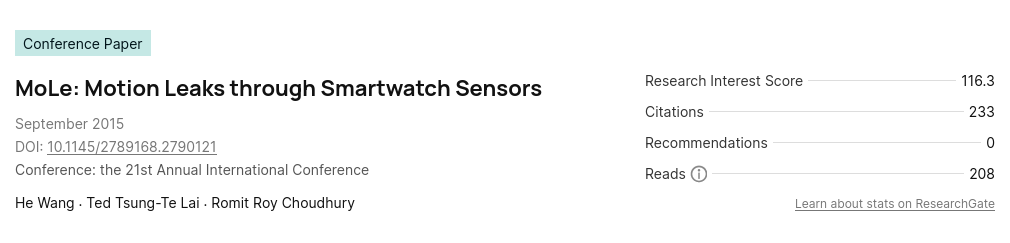
\includegraphics[width=1\linewidth]{imgs/MoLePaper}
\end{frame}


\begin{frame}
 \begin{itemize}
 	\item The paper highlights the significant ramifications
 	of such data leakage, as smartwatches can be camouflaged
 	as activity trackers, thereby compromising the privacy of a
 	\textbf{user’s emails, search queries, and other documents typed} on
 	the keyboard. 
 	
 	%Given the importance of addressing privacy and  	security risks associated with accelerometer data, this paper  	has been selected for further investigation and analysis.
 	\item %Unlike keystroke loggers that need to find loopholes in the 	operating system, 
 	The activity tracker malware can obtain the	user’s permission and easily launch a side channel attack. 	
 \end{itemize}
\end{frame}

\begin{frame}{Assumptions and Constraints}
	\begin{itemize}
		\item Smartwatch is worn on the left hand.
		\item The absence of data from the right hand is a unique constraint, and so it needs to infer which finger	executed the key-press.
		\item For a given position of the wrist watch, it is not obvious which one of the 3 or 4 different keys could have been pressed, which could be further interspersed by unknown number of keys pressed by the right hand. 
		\item Users write different with dexterity, e.g. some use their little
		finger far less efficiently while others use specific fingers when
		it comes to digits or corner keys.
	\end{itemize}
\end{frame}

\begin{frame}{Data Collection}
	\begin{itemize}
		\item \textbf{Training data:} Two authors put on Samsung Gear Live
		smart watches and typed 500 words recording the accerlerometer and gyroscope data.
		\item The training data is processed through a sequence of steps, including key-press detection, hand-motion tracking,
		character point cloud computation, and Bayesian modeling and
		inference.
		\item The \textbf{test data} was collect by 8 different volunteers
		who were asked to type 300 different English words from a
		dictionary.
		\item The smart-watch sensor data from the volunteers
		was used to create a short-lists $K$ words, ranked in the
		decreasing order of probability (i.e., the first ranked word is
		considered the most probable guess.
	\end{itemize}	
\end{frame}


\begin{frame}{Collection Procedure}
	
\begin{minipage}[c]{0.49\linewidth}
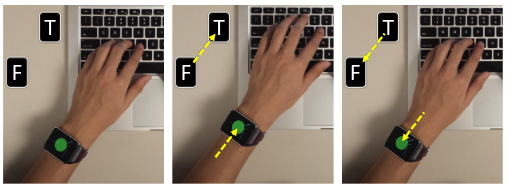
\includegraphics[width=\textwidth]{imgs/watchMovement}
%Two of the authors wore a smartwatch and recorded the accelerometer and gyroscope data as they typed each character one by one. The positive $X$ axis of the watch is parallel to the arm and pointed towards the fingers, the positive $Y$ axis is perpendicular and upward, and the positive $Z$ axis pointed upwards from the plane of the arm.

%In order to collect the ground truth data, a phone camera was placed right on top of the keyboard and recorded video at 30 fps and smart watch movements were captured by computer vision techniques.  
% The watch, the phone camera, and the keyboard loggerwere all time–synchronized via the network time protocol (NTP).The synchronization offers precise correspondence between the sensor and visual data, extending semantic meaning to the motion signals.
%Figure \ref{watchMovements} shows an example sequence of video frames capturing the process of typing the character \enquote{T}. The left hand starts from a home position (i.e., the key \enquote{F}), moves along the $+X$ direction to press \enquote{T}, hits the key, and returns back to the home position.  The yellow arrow on the arm shows the displacement of the green marker on the watch.
\end{minipage}
\begin{minipage}[c]{0.49\linewidth}
	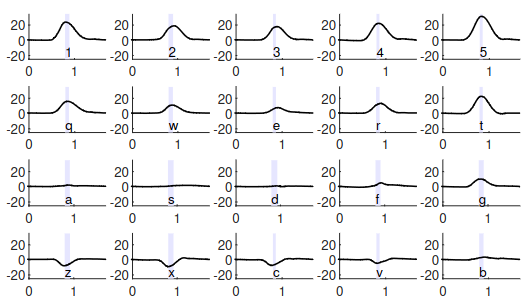
\includegraphics[width=\textwidth]{imgs/mobicom}
	% In Figure 6, motion data from 20 different characters	located on the left side of the keyboard is plotted. Each 	graph shows the displacement of the watch computed from the	accelerometer’s X axis data, with the X axis representing time 	and the Y axis representing displacement. The accelerometer’s	Y and Z axes are not shown. The time of the key-press, 	obtained from the keyboard logger, is marked by a light 	gray vertical bar in each graph. It can be observed that the 	displacements align well with the layout of the keyboard. The 	first row (12345) generates the largest positive displacement, 	while the last row (zxcvb) produces negative displacement. 	As the left fingers are initially placed on the third row (asdf), 	nearly no displacement is detected for these characters. The 	authors suggest that although this is preliminary research, 	these signals provide the first indication of information leakage 	through smartwatches.
\end{minipage}

\begin{minipage}[c]{0.49\linewidth}
	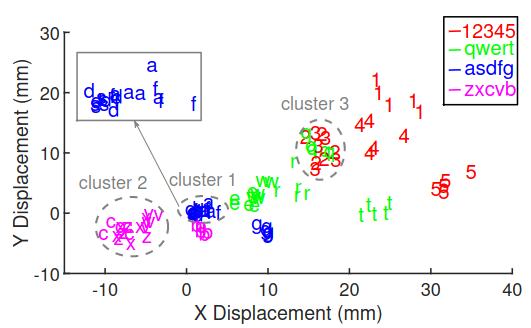
\includegraphics[width=\textwidth]{imgs/displacement}
	% In Figure \ref{displacement}, the watch displacement for the same 20 keys is shown in 2D space using the combined $X$ and $Y$ axes data from the accelerometer. Each color represents one row on the keyboard. Some keys, such as 1, t, r, 4, and 5, are quite isolated, while others overlap strongly, particularly "asdf," "zxcv," and "q23" exhibit the strongest overlaps. This is not surprising since the cluster "asdf" is an outcome of the fingers being on these keys in the home position, and the wrist hardly needs to move when typing these keys. Similarly, the fingers move uniformly downward for "zxcv," resulting in similarity between the keys. Lastly, the hand movement for "q" is similar to "2" and "3," even though they are not on the same row. This is because the little finger is shorter, and to type the character "q," it must move as much as the ring finger must move to type "2."
\end{minipage}
\begin{minipage}[c]{0.49\linewidth}
	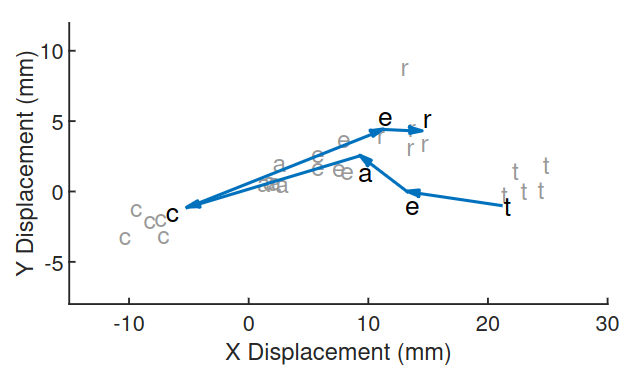
\includegraphics[width=\textwidth]{imgs/displacement2}
	% Decoding characters becomes more complex when the user types a word rather than just a single character. Figure \ref{displacement2} displays the sequence of hand displacements when the word "teacher" is typed. Obvious issues arise: The wrist motion for each character is no longer aligned with the earlier observations since the motion is relative to the previous position of the key. It can be observed that "e," "a," and "c" are all far away from their respective clusters detected earlier in Figure \ref{displacement}. Additionally, "h" (pressed by the right hand) was not recorded, and instead, a small random motion of the left hand during this time was captured. Finally, real-world environments do not have cameras, so the data is completely unlabeled. A wrong decision about any of the keys can derail all subsequent decisions. In conclusion, while sensor data from smartwatches can encode the human-typed information, decoding them reliably in real-world conditions presents non-trivial challenges.
	
\end{minipage}
Figures are taken from \cite{b1}.
\end{frame}


\begin{frame}{MoLe: Overview}
	\begin{figure}
	\centering
	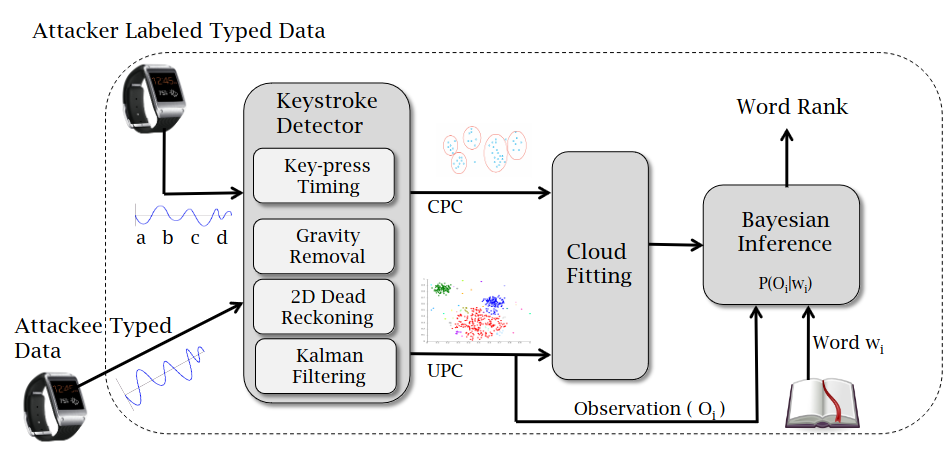
\includegraphics[width=1\linewidth]{imgs/moleOverview}
	\caption{Figure is taken from \cite{b1}.}
	\end{figure}
	
	% Figure \ref{moleOverview} illustrates the flow of operations in the end to end MoLe 	system. At the backend server, the attacker types each character 	 	on a computer keyboard multiple times and computes a character point cloud (CPC) similar to the one in Figure \ref{displacement}. The operation is performed offline, and is stored separately for use later.
	
	%The process of decoding the raw sensor data involves passing it through a module called %"Keystroke Detection", which has two tasks. Firstly, it detects the timing of each keystroke by analyzing the $Z$ axis of the sensor data, where a negative dip in the $Z$ axis corresponds to a key press. Secondly, it computes the net 2D displacement of the watch by processing the signal through several steps, including gravity and mean removal, double integration, and Kalman Filtering. The output of this module is a set of tuples representing the estimated location of the watch at the time of each key press. These tuples form an unlabeled point cloud (UPC) on a 2D plane. The UPC is then passed to the "Cloud Fitting" module, which assigns approximate labels to the points by scaling and rotating the convex hull of a previously computed character point cloud (CPC) to best fit the convex hull of the UPC. This rotated and scaled CPC serves as the reference template for decoding the unlabeled points in the UPC. 
	
	%The \enquote{Cloud Fitting} module receives the UPC and its primary responsibility is to provide estimated labels for the points in the UPC. To achieve this, the module uses the previously computed CPC and adjusts the scaling and rotation of the CPC's convex hull to match the convex hull of the UPC as closely as possible. The resulting rotated and scaled CPC serves as a reference template for identifying the characters corresponding to the unlabeled points in the UPC
	
	%The \enquote{Bayesian Inference} module takes in three inputs: (1) the template output from Cloud Fitting, (2) the unlabeled points from the UPC, and (3) a dictionary $W$ of valid English words. For each valid word $w_i$ in the dictionary, the module computes the a posteriori probability that the unlabeled points form $w_i$. This is done by computing the probability that each unlabeled point corresponds to a specific character in the word. The product of these probabilities is the final probability that the unlabeled points form the word $w_i$. The module computes this probability for each word $w_i$ and outputs a ranked list of $\textless$word, probability$\textgreater$ tuples as a guess of the user-typed word.
	%If the input is a password, the attacker can try out all the guesses above some probability threshold. If the input is an email or a search query, the attacker could manually try to decode the text from the possible sets of words. Even though MoLe does not offer a single suggestion, the probability estimate associated with each guess dramatically reduces the search space for the attacker.	
	
\end{frame}


\begin{frame}{Constraints}
	This paper defines the following conditions for their experiment:
	\begin{itemize}
		\item Volunteers type one word at a time (as opposed to free-flowing
		sentences).
		\item Only valid English words are allowed. Passwords that contain interspersed digits, or non-English character-sequences, are not decodable as of now.
		\item  The same Samsung smart watch model was used for both
		the attacker and the user.
		\item They assumed the user is seasoned in typing in that he/she roughly
		uses the appropriate fingers – novice typists who do not abide by
		basic typing rules may not be subject to our proposed attacks.
	\end{itemize}
\end{frame}



\begin{frame}{Keystroke Detector}
	
	%This module is tasked with computing the timing and position of each key press present in the sensor signals. The position is represented by a 2D vector with the origin at the "F" key on the keyboard. Collecting all of the key press positions will result in the point cloud as discussed previously.
	
	\begin{minipage}[c]{0.49\linewidth}
		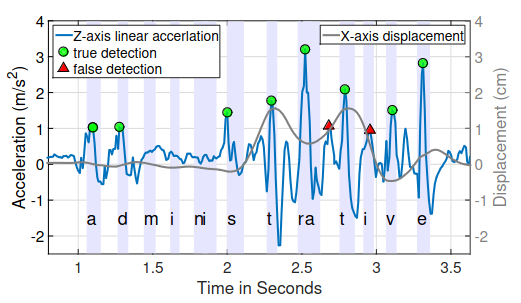
\includegraphics[width=\textwidth]{imgs/peakdetection}
		% The method to detect key presses is based on the idea that when a finger is pressed on a key, the wrist undergoes a partial dipping motion which can be observed in the $Z$-axis of the watch. The $Z$-axis motion when a user types the word "administrative" is shown in Figure \ref{peakdetection}. Although actual key presses generally produce prominent peaks, false positives and false negatives can occur. False positives are mainly observed during transitions between keys, where the hand moves up slightly before making the movement, which can be reflected in the $Z$-axis motion. False negatives are usually due to subtle $Z$-axis motion for keys like "asdf" that may not be detected. Ground truth is used to observe these false positives and false negatives.
	\end{minipage}
	\begin{minipage}[c]{0.49\linewidth}
		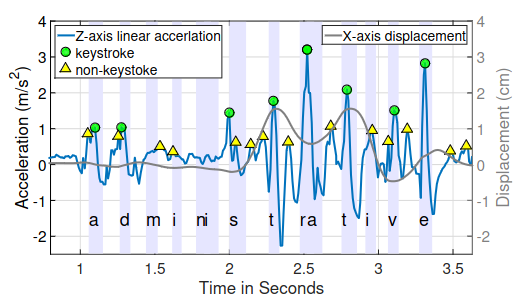
\includegraphics[width=\textwidth]{imgs/baggedDecision}
		% To address false positives and false negatives when detecting keystrokes, bagged decision trees are used as an ensemble classifier that trains multiple decision trees by selecting different subsets of features and training examples. This approach improves the stability and accuracy by letting each subtree learn on the attacker's labeled data, apply the learning to the unlabeled data, and then compute the final results via voting.
		% To obtain labeled data, a simple threshold-based peak detection method is applied on the $Z$-axis acceleration, and true/false detection is labeled on the attacker's template. The peak detection threshold is set to be low so as not to miss true keystrokes. Features are extracted within a time window around the labels, and the classifier is trained using these features.
		
		%The feature set includes various metrics such as width, height, and prominence of the $Z$-axis peak, mean, variance, max, min, skewness, and kurtosis for each of the 3-axis displacement, velocity, acceleration, and gyroscope rotation, the magnitude of acceleration/gyroscope, and the correlation of each pair between acceleration and gyroscope vectors.
		%When the attacker's sensor data arrives, the same peak detection scheme is applied, and many candidate keystrokes and their features are obtained. The classifier identifies the validity of the keystroke and selects the maximum value of $Z$-axis acceleration to denote the timing of the key-press. An example of the classification result for the word "administrative" is shown in Figure \ref{baggedDecision}.
		
	\end{minipage}	
\centering \tiny
Figures are taken from \cite{b1}.
\end{frame}

\begin{frame}{Key-press location}
	\begin{figure}
		\centering
		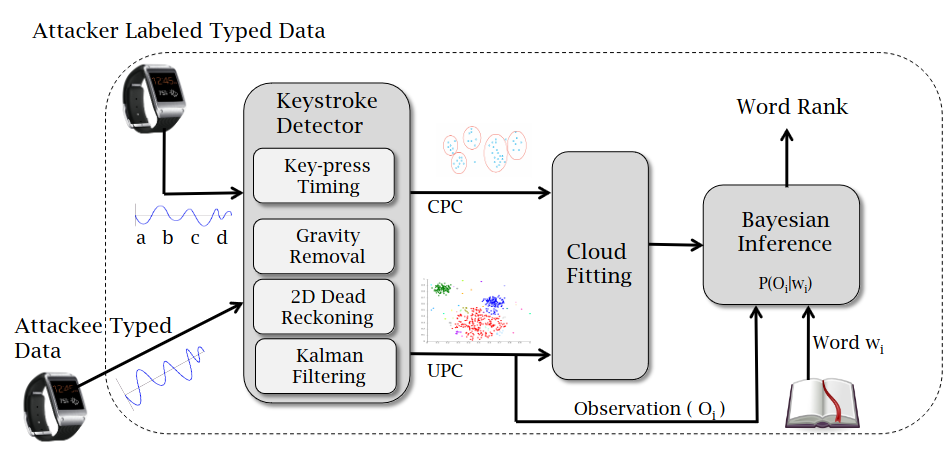
\includegraphics[width=10cm]{imgs/moleOverview}
		\caption{Figure is taken from \cite{b1}.}
	\end{figure}
	% The primary challenge is accurately tracking hand motion during key transitions to determine key-press locations. 
	%It requires high accuracy, as errors can cascade. 
	%The left index finger's periodic return to the home key "F" allows recalibration and improves tracking accuracy. Initially, Android API's linear acceleration data was used but it was unsatisfactory. So the authors developed a tailored tracking approach by themselves. 
	\begin{itemize}
		\item Steps include finding gravity to establish an absolute coordinate system, estimating and removing gravity using gyroscope data, estimating coordinates and calculating projected acceleration, and calibrating speed and displacement through mean removal. 
		\item A Kalman smoothing was also employed for displacement estimation stability.
	\end{itemize}
\end{frame}


\begin{frame}{Point Cloud Fitting}
	\begin{figure}
		\centering
		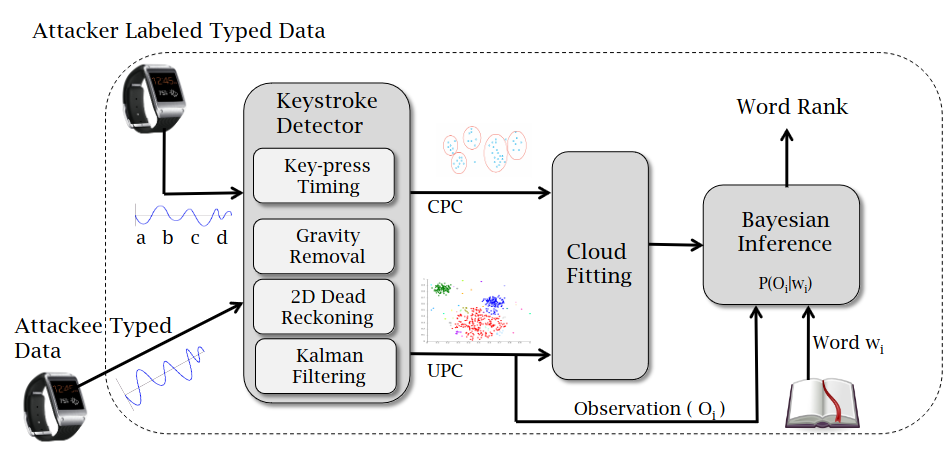
\includegraphics[width=10cm]{imgs/moleOverview}
		\caption{Figure is taken from \cite{b1}.}
	\end{figure}
	\begin{itemize}
		\item 
	\end{itemize}
	% MoLe generates an unlabeled point cloud (UPC) based on the estimated displacements for each key pressed by the attacker. To assign approximate labels to the points in the UPC, MoLe fits the attacker's character point cloud (CPC) to the UPC. The fitting process involves computing convex hulls for both the CPC and the UPC.
	%MoLe computes two convex hulls for the CPC, one for positive $X$ displacements ($H^{CPC}_{pos}$) and another for negative $X$ displacements ($H^{CPC}_{neg}$). Similarly, two convex hulls are computed for the UPC ($H^{CPC}_{pos}$ and $H^{UPC}_{neg}$). The fitting is performed by rotating and scaling the CPC's convex hulls to align with the UPC's convex hulls. The fitting metric is based on the degree of overlap between the two convex hulls, specifically the ratio of their intersection and union.
	%In cases where the attacker generates multiple CPCs, MoLe performs the fitting process for each CPC and selects the one that maximizes the intersection/union ratio. Once the CPC is rotated and scaled, it is superimposed on the UPC, creating a framework for estimating labels for each point in the UPC.
\end{frame}






\begin{frame}{Bayesian Inference}
\begin{figure}
	\centering
	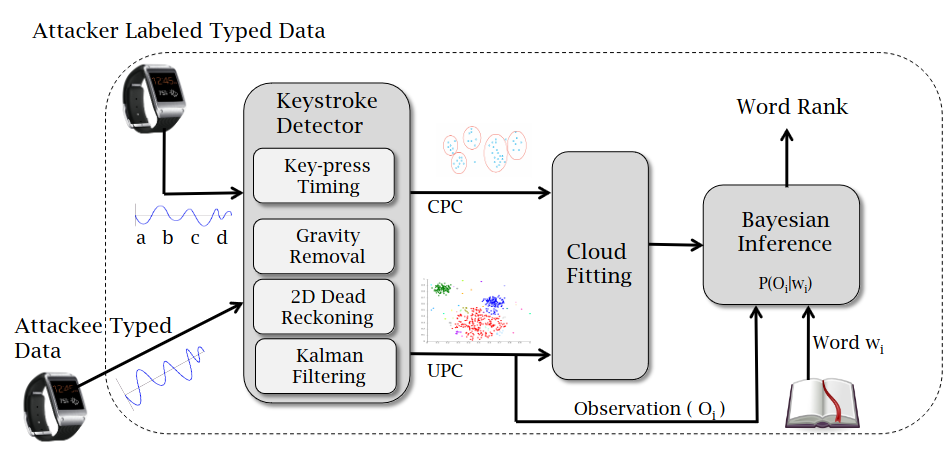
\includegraphics[width=10cm]{imgs/moleOverview}
	\caption{Figure is taken from \cite{b1}.}
\end{figure}
		% After detecting keystrokes and fitting the point cloud, MoLe aims to infer the characters typed by the right hand, filling in the missing information. One approach is to calculate the posterior probability of each word in the English dictionary given the motion inferences from the left hand.
	%The Bayesian inference step involves calculating the posterior probability of each word in the English dictionary given the observed motion data from the left hand. The likelihood function estimates the probability of each word based on the observed motion data, and the prior probability captures the word's occurrence frequency. By applying Bayes' theorem, the posterior probability is obtained. The goal is to find the word with the highest likelihood given the observed data. Various refinements can be applied to improve the likelihood function and posterior probability estimation.
	%One approach is to consider the number of detected keystrokes as observations to match the word. The number of keys typed by the left hand is used to evaluate the likelihood of each word. Additionally, for cases where two consecutive characters are detected as a single keystroke due to close succession, treating them as one key-press can be appropriate. These refinements enhance the accuracy of word matching based on the observed motion data.
	%Another refinement in the Bayesian inference step involves incorporating language models to estimate the likelihood of words based on the observed motion data. Language models can capture the statistical patterns and probabilities of word sequences in a given language. By considering the context and word probabilities, the likelihood function can be further refined, leading to more accurate posterior probability estimation. This enhancement leverages linguistic information to improve the matching of observed motion data with candidate words from the dictionary.
\end{frame}



\begin{frame}{Setup Test Data}
\begin{itemize}
	\item Accelerometer and gyroscope readings were recorded at 200Hz on the Galaxy Gear Live smartwatch.
	%\item The sensor data is stored locally during data collection and later transferred to a backend MATLAB server for analysis.
	\item 	Eight volunteers were recruited familiar with English typing, each typed 300 English words randomly selected from the 5000 most frequently used words. % A total of 2400 words were tested across all users.
	%\item The word length ranged from 1 to 14, and each length was equally distributed.
	%\item During the experiment, subjects were seated at a desk in front of a Lenovo laptop.
	\item A word appeared one at a time on the laptop screen, and the subjects were instructed to type the same word in a text box on the screen.
	\item If any characters were mistyped, the data was discarded, and the subject was asked to re-enter the word. 
	\item Subjects were instructed to initialize their hand position on the "F" and "J" keys between each word recording. 
	\item The laptop recorded the timing of the keystrokes, which served as the ground truth.
\end{itemize}
\end{frame}

\begin{frame}{Setup Training Data}
	\begin{itemize}
		\item To collect training data, two of the authors acted as attackers and followed the \textbf{same procedure}, but with the top 500 longest words in the dictionary.
		%The use of long words helped capture a diverse range of typing patterns. 
		%The data collection for the offline training was done using a Lenovo ThinkPad equipped with a regular full-sized keyboard.
		\item For full ground truth recording, an Android Samsung Galaxy S4 phone was mounted on top of the keyboard, and the front camera was used to capture video of hand movement. 
		\item The camera calibration toolbox in MATLAB was used to calibrate the camera pixel and measure the watch distance and location from each frame.
	\end{itemize}
\end{frame}


\begin{frame}{Cumulative Distribution Function of Rank}
\begin{figure}
	\centering
	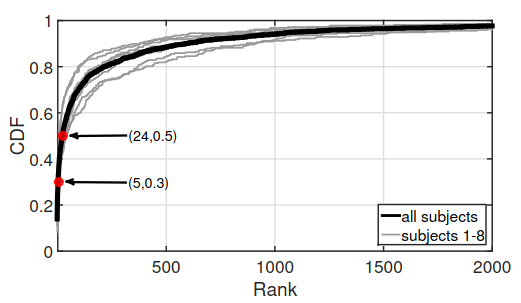
\includegraphics[width=7cm]{imgs/cdfInferTyped.png}
	\caption{Figure is taken from \cite{b1}.}
\end{figure}
	
\begin{itemize}
	\item Figure illustrates the cumulative distribution function (CDF) of rank. %, based on the analysis of 2400 words typed by the subjects in the experiments. 
	%	\item The black line represents the average performance across all 8 subjects, while the gray lines represent MoLe's performance for each individual subject. 
	 \item The results indicate that the median rank of a word is 24, i.e. there is a 50\% chance that MoLe can narrow down the typed word to 24 possibilities. 
	 \item At the 30th percentile, the rank is 5, indicating a 30\% chance of narrowing down the possibilities to \textbf{just 5 words}. % This reduction in the search space, considering a total of 5000 possible words, is significant and increases susceptibility to brute-force attacks.
\end{itemize}
\end{frame}


 
 \begin{frame}
 	\begin{figure}
 		\centering
 		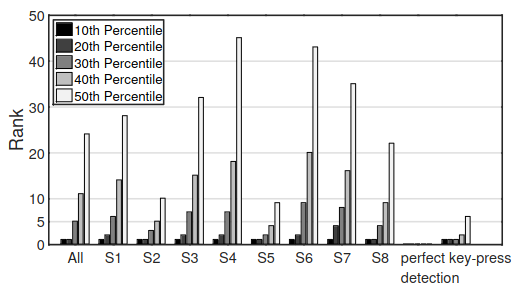
\includegraphics[width=7cm]{imgs/RankOfAverage.png}
 		\caption{Figure is taken from \cite{b1}.}
 	\end{figure}
 \begin{itemize}
	 \item Figure displays the ranks of typed words for each test subject.
	 %It is observed that subjects S2, S5, and S8 generally have higher ranks, indicating that MoLe's guesses are more accurate for these individuals. Upon analyzing the video and sensor traces, it is discovered that these subjects exhibit lower variance in their hand movements, likely due to adhering to the prescribed typing guidelines.
	 % Furthermore, a test is conducted with perfect key-press detection, utilizing the actual number and timing of keystrokes from the left hand, obtained from the ground truth timing information. Surprisingly, the 30th percentile drops to 1, indicating that MoLe can precisely guess the word, and the 50th percentile drops to 6. This outcome highlights that further enhancements in key-press detection are crucial for the improvement of MoLe's performance.
	 \item When the left character count ranges from 2 to 4, the performance of MoLe tends to degrade. % This is because there are many words that share the same 2 to 4 left-hand characters. The similarity in the initial characters makes it more difficult for MoLe to accurately narrow down the possibilities and correctly identify the typed word.
	 
	\item  The rank generally decreases as the word length exceeds 6. 
	%This is primarily due to two reasons. Firstly, longer words tend to have a greater number of keystrokes, which increases the chances of accurate detection. Secondly, the number of words with longer lengths decreases, reducing the possibilities for confusion.
	 
	\item Conversely, words with lengths ranging from 4 to 7 have fewer keystrokes, making them more challenging to detect. 
	% Additionally, there are a larger number of words with these lengths, further adding to the difficulty of detection.
	
	%MoLe’s ability to guess degrades drastically with lower sampling rates (200Hz, 100Hz, 50Hz, 20H) – median ranking falls as 64, 141 and 1218.
	
	\item  The authors state that the system performance is close between two keyboards, even though 	the attackers used the laptop keyboard for training the system. 
	
 \end{itemize}
 \end{frame}
 


\begin{frame}{Example}
	\begin{figure}
		\centering
		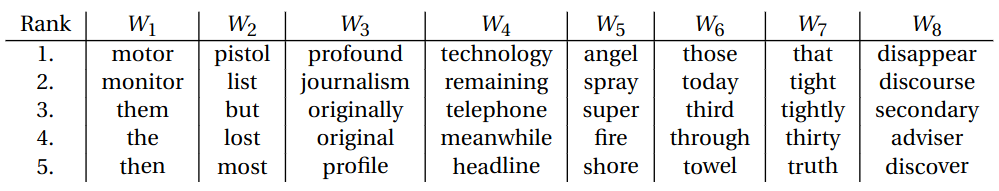
\includegraphics[width=\linewidth]{imgs/sentence.png}
		\caption{Table is taken from \cite{b1}.}
	\end{figure}

\begin{itemize}
 	\item Table displays MoLe's end-to-end prediction results for each word in an actual sentence entered by subject S5. 
 	\item The table lists the Top-5 guesses for each word, with the most likely guess at the top. \item The words in each column exhibit similarity in their character sequences. 
 	\pause 
 	\item By examining the table, readers can reconstruct the sentence: \alert{The most profound technologies are those that disappear}.

\end{itemize}
\end{frame}


\begin{frame}{Limitations}
\begin{itemize}
	\item MoLe is not able to infer non-valid English words, such as passwords.
\item There is no scalability across different watch models.
\item Training and test data contain no mistake such as mistyping and pressing delete key.
\item Subjects were instructed to follow the typing guideline such as returning to "F"-Key.
\item It is capable to parse sentences due to difficulties in detecting the "space bar".
\item Despite the authors' assertion that the disparity between the two keyboards is minimal, their evaluation was limited to testing only two selected models.
\item However, the authors state that although no tests were made with other wearable devices such as Fitbits, they believe with some customization, the attacks can be launched on those platforms as well.
\end{itemize}
	\pause 	
	\begin{alertblock}{Note}
		MoLe is not yet a real-world attack.
	\end{alertblock}
\end{frame}






\section*{Summary}

\begin{frame}{Take Home Messages}

  % Keep the summary *very short*.
  \begin{itemize}
  \item
    The \alert{first main message} of your talk in one or two lines.
  \item
    The \alert{second main message} of your talk in one or two lines.
  \item
    Perhaps a \alert{third message}, but not more than that.
  \end{itemize}
\end{frame}



% All of the following is optional and typically not needed. 
\appendix
\section<presentation>*{\appendixname}
\subsection<presentation>*{For Further Reading}

\begin{frame}[allowframebreaks]
  \frametitle<presentation>{For Further Reading}
    
  \begin{thebibliography}{10}
   
  
  %\beamertemplatebookbibitems
  % Start with overview books.

%  \bibitem{Author1990}
 %   A.~Author.
  %  \newblock {\em Handbook of Everything}.
   % \newblock Some Press, 1990.
 	
    
  \beamertemplatearticlebibitems
  % Followed by interesting articles. Keep the list short. 
	
\bibitem{b1} Seneviratne, Suranga et al. “A Survey of Wearable Devices and Challenges.” IEEE Communications Surveys \& Tutorials 19 (2017): 2573-2620.
\bibitem{b2} Delgado-Santos, Paula et al. “A Survey of Privacy Vulnerabilities of Mobile Device Sensors.” ACM Computing Surveys (CSUR) 54 (2022): 1 - 30.
\bibitem{b3} Wang, He et al. “MoLe: Motion Leaks through Smartwatch Sensors.” Proceedings of the 21st Annual International Conference on Mobile Computing and Networking (2015): n. pag.
\bibitem{b4} Liu, Xiangyu et al. “When Good Becomes Evil: Keystroke Inference with Smartwatch.” Proceedings of the 22nd ACM SIGSAC Conference on Computer and Communications Security (2015): n. pag.
\bibitem{b5} Kröger, Jacob Leon et al. “Privacy implications of accelerometer data: a review of possible inferences.” Proceedings of the 3rd International Conference on Cryptography, Security and Privacy (2019): n. pag.

% Just for citing
\bibitem{b6} R. Goyal, N. Dragoni, and A. Spognardi, “Mind the tracker You wear:
A security analysis of wearable health trackers,” in Proceedings of the
31st Annual ACM Symposium on Applied Computing, ser. SAC ’16.
New York, NY, USA: ACM, 2016, pp. 131–136.
\bibitem{b7} https://openeffect.ca/reports/Every\_Step\_You\_Fake.pdf, 2016.
    
    
  \bibitem{smartwatches}
  \url{https://cdn.test.de/file/image/87/08/0404382e-ad12-4c12-b8e8-906f8e2d37c7-web/6003370_smartwatches-t202306;a3-2.jpg} 
  \end{thebibliography}
\end{frame}

\end{document}
